\begin{figure}
    \centering
    \begin{subfigure}{0.45\textwidth}
        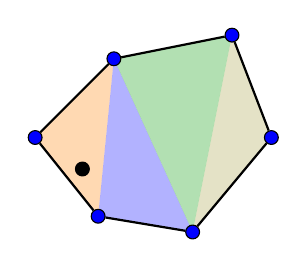
\begin{tikzpicture}
        \coordinate (a) at (0,0);
        \coordinate (b) at (1, 1);
        \coordinate (c) at (2.5, 1.3);
        \coordinate (d) at (3, 0);
        \coordinate (e) at (0.8, -1);
        \coordinate (f) at (2, -1.2);

        \fill[orange, opacity=0.3] (a) -- (b) -- (e) -- (a) -- cycle;
        \fill[blue, opacity=0.3] (b) -- (f) -- (e) -- (b) -- cycle;
        \fill[green!60!black, opacity=0.3] (b) -- (c) -- (f) -- (b) -- cycle;
        \fill[yellow!60!black, opacity=0.3] (c) -- (d) -- (f) -- (c) -- cycle;
       
        \node[draw, circle, black, fill=blue, inner sep=0pt, minimum size=5pt] (pA) at (0, 0) {};
        \node[draw, circle, black, fill=blue, inner sep=0pt, minimum size=5pt] (pB) at (1, 1) {};
        \node[draw, circle, black, fill=blue, inner sep=0pt, minimum size=5pt] (pC) at (2.5, 1.3) {};
        \node[draw, circle, black, fill=blue, inner sep=0pt, minimum size=5pt] (pD) at (3, 0) {};
        \node[draw, circle, black, fill=blue, inner sep=0pt, minimum size=5pt] (pE) at (0.8, -1) {};
        \node[draw, circle, black, fill=blue, inner sep=0pt, minimum size=5pt] (pF) at (2, -1.2) {};

        \node[draw, circle, black, fill=black, inner sep=0pt, minimum size=5pt] (pG) at (0.6, -0.4) {};

        
        \draw[thick] (pA) -- (pB) -- (pC) -- (pD) -- (pF) -- (pE) -- (pA);
        % \draw[dashed, thick, red] (pA) -- (pB) -- (pE) -- (pA);
        % \draw[dashed, thick, blue] (pB) -- (pF) -- (pE) -- (pB);
        % \draw[dashed, thick, green!60!black] (pB) -- (pC) -- (pF) -- (pB);

        
        \end{tikzpicture}
        \caption{}
    \end{subfigure}
    \begin{subfigure}{0.45\textwidth}
        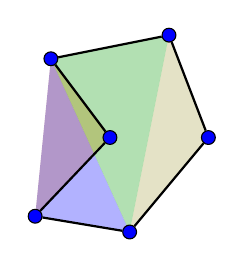
\begin{tikzpicture}
            \coordinate (a) at (1.75,0);
            \coordinate (b) at (1, 1);
            \coordinate (c) at (2.5, 1.3);
            \coordinate (d) at (3, 0);
            \coordinate (e) at (0.8, -1);
            \coordinate (f) at (2, -1.2);
    
            \fill[orange, opacity=0.3] (a) -- (b) -- (e) -- (a) -- cycle;
            \fill[blue, opacity=0.3] (b) -- (f) -- (e) -- (b) -- cycle;
            \fill[green!60!black, opacity=0.3] (b) -- (c) -- (f) -- (b) -- cycle;
            \fill[yellow!60!black, opacity=0.3] (c) -- (d) -- (f) -- (c) -- cycle;
           
            \node[draw, circle, black, fill=blue, inner sep=0pt, minimum size=5pt] (pA) at (1.75, 0) {};
            \node[draw, circle, black, fill=blue, inner sep=0pt, minimum size=5pt] (pB) at (1, 1) {};
            \node[draw, circle, black, fill=blue, inner sep=0pt, minimum size=5pt] (pC) at (2.5, 1.3) {};
            \node[draw, circle, black, fill=blue, inner sep=0pt, minimum size=5pt] (pD) at (3, 0) {};
            \node[draw, circle, black, fill=blue, inner sep=0pt, minimum size=5pt] (pE) at (0.8, -1) {};
            \node[draw, circle, black, fill=blue, inner sep=0pt, minimum size=5pt] (pF) at (2, -1.2) {};
    
            % \node[draw, circle, black, fill=black, inner sep=0pt, minimum size=5pt] (pG) at (0.6, -0.4) {};
    
            
            \draw[thick] (pA) -- (pB) -- (pC) -- (pD) -- (pF) -- (pE) -- (pA);
            % \draw[dashed, thick, red] (pA) -- (pB) -- (pE) -- (pA);
            % \draw[dashed, thick, blue] (pB) -- (pF) -- (pE) -- (pB);
            % \draw[dashed, thick, green!60!black] (pB) -- (pC) -- (pF) -- (pB);
    
    
        \end{tikzpicture}
        \caption{}
    \end{subfigure}
    \caption{Illustration of the proof for \lstinline|ConvexEmptyIn.iff_triangles|. The left subfigure shows how a point inside the polygon implies the point is inside one of the triangles of triangulation of its convex hull. The right subfigure shows how non-convexity implies one of the vertices of the polygon will be inside one of the triangles of the convex hull partition.}\label{fig:triangulation}
\end{figure}